% 请确保文件编码为utf-8,使用XeLaTex进行编译,或者通过overleaf进行编译

\documentclass[answers]{exam}  % 使用此行带有作答模块
% \documentclass{exam} % 使用此行只显示题目

\usepackage{xeCJK}
\usepackage{zhnumber}
\usepackage{graphicx}
\usepackage{hyperref}
\usepackage{amsmath}
\usepackage{booktabs}
\usepackage{enumerate}
\usepackage{amssymb}
\usepackage{listings}
\usepackage{floatrow}
\usepackage{blindtext}
\pagestyle{headandfoot}
\firstpageheadrule
\firstpageheader{南京大学}{机器学习导论}{习题二}
\runningheader{南京大学}
{机器学习导论}
{习题二}
\runningheadrule
\firstpagefooter{}{第\thepage\ 页(共\numpages 页)}{}
\runningfooter{}{第\thepage\ 页(共\numpages 页)}{}


\setlength\linefillheight{.5in}

\renewcommand{\solutiontitle}{\noindent\textbf{解:}\par\noindent}

\renewcommand{\thequestion}{\zhnum{question}}
\renewcommand{\questionlabel}{\thequestion .}
\renewcommand{\thepartno}{\arabic{partno}}
\renewcommand{\partlabel}{\thepartno .}

\lstset{language=Matlab}%这条命令可以让LaTeX排版时将Matlab关键字突出显示
\lstset{
	breaklines,%这条命令可以让LaTeX自动将长的代码行换行排版
	basicstyle=\footnotesize\ttfamily, % Standardschrift
	backgroundcolor=\color[rgb]{0.95,0.95,0.95},
	keywordstyle=\color{blue},
	commentstyle=\color{cyan},
	tabsize=4,numbers=left,
	numberstyle=\tiny,
	frame=single,
	%numbers=left, % Ort der Zeilennummern
	numberstyle=\tiny, % Stil der Zeilennummern
	%stepnumber=2, % Abstand zwischen den Zeilennummern
	numbersep=5pt, % Abstand der Nummern zum Text
	tabsize=2, % Groesse von Tabs
	extendedchars=false, %
	breaklines=true, % Zeilen werden Umgebrochen
	keywordstyle=\color{red},%这一条命令可以解决代码跨页时, 章节标题, 页眉等汉字不显示的问题
	stringstyle=\color{white}\ttfamily, % Farbe der String
	showspaces=false, % Leerzeichen anzeigen ?
	showtabs=false, % Tabs anzeigen ?
	xleftmargin=17pt,
	framexleftmargin=17pt,
	framexrightmargin=5pt,
	framexbottommargin=4pt,
	%backgroundcolor=\color{lightgray},
	showstringspaces=false % Leerzeichen in Strings anzeigen ?
}
\renewcommand{\lstlistingname}{CODE}
\lstloadlanguages{% Check Dokumentation for further languages ...
	%[Visual]Basic
	%Pascal
	%C
	Python
	%XML
	%HTML
	%Java
}
%%% load AMS-Latex Package
\usepackage{amssymb}
\usepackage{amsmath,amsfonts}
% \usepackage{amsthm}
\usepackage{amsopn}
\usepackage{bm} % bold symbol
\usepackage{multirow}



% operator in optimization
\DeclareMathOperator{\argmax}{arg\,max}
\DeclareMathOperator{\argmin}{arg\,min}
\DeclareMathOperator{\softmax}{softmax}

% special functions
\newcommand{\trace}[1]{\operatornamewithlimits{tr}\left\{#1\right\}}
\newcommand{\diag}{\operatornamewithlimits{diag}}
\newcommand{\sign}{\operatornamewithlimits{sign}}
\newcommand{\const}{\operatornamewithlimits{const}}

% special display
\newcommand{\parde}[2]{\frac{\partial #1}{\partial  #2}}

% define vector and matrix symbols
\newcommand{\vct}[1]{\boldsymbol{#1}} % vector
\newcommand{\mat}[1]{\boldsymbol{#1}} % matrix
\newcommand{\cst}[1]{\mathsf{#1}}  % constant

% shorthand
\newcommand{\vtheta}{\vct{\theta}}
\newcommand{\vmu}{\vct{\mu}}
\newcommand{\vc}{\vct{c}}
\newcommand{\vp}{\vct{p}}
\newcommand{\vq}{\vct{q}}
\newcommand{\vx}{{\vct{x}}}
\newcommand{\vy}{\vct{y}}
\newcommand{\vz}{{\vct{z}}}
\newcommand{\vu}{\vct{u}}
\newcommand{\vo}{{\vct{o}}}
\newcommand{\va}{\vct{a}}
\newcommand{\vb}{\vct{b}}
\newcommand{\ve}{\vct{e}}
\newcommand{\vr}{\vct{r}}
\newcommand{\vt}{\vct{t}}
%\newcommand{\vpsi}{\vct{\psi}}
\newcommand{\vs}{\vct{s}}
\newcommand{\vv}{\vct{v}}
\newcommand{\vw}{\vct{w}}
\newcommand{\vzero}{\vct{0}}
\newcommand{\vf}{\vct{f}}
\newcommand{\vh}{\vct{h}}
\newcommand{\vg}{\vct{g}}
\newcommand{\vphi}{\vct{\phi}}
\newcommand{\vpsi}{\vct{\psi}}
\newcommand{\ones}{\vct{1}}
\newcommand{\mU}{\mat{U}}
\newcommand{\mA}{\mat{A}}
\newcommand{\mB}{\mat{B}}
\newcommand{\mC}{\mat{C}}
\newcommand{\mD}{\mat{D}}
\newcommand{\mV}{\mat{V}}
\newcommand{\mW}{\mat{W}}
\newcommand{\mH}{\mat{H}}
\newcommand{\mI}{\mat{I}}
\newcommand{\mP}{\mat{P}}
\newcommand{\mS}{\mat{S}}
\newcommand{\mJ}{\mat{J}}
\newcommand{\mM}{\mat{M}}
\newcommand{\mT}{\mat{T}}
\newcommand{\mZ}{\mat{Z}}
\newcommand{\mO}{\mat{O}}
\newcommand{\mX}{\mat{X}}
\newcommand{\mY}{\mat{Y}}
\newcommand{\mQ}{\mat{Q}}
\newcommand{\mLambda}{\mat{\Lambda}}
% \newcommand{\mL}{\mat{L}}
\newcommand{\mmI}{\mat{I}}
\newcommand{\mK}{\mat{K}}
\newcommand{\mSigma}{\mat{\Sigma}}
\newcommand{\mOmega}{\mat{\Omega}}
\newcommand{\cC}{\cst{C}}
\newcommand{\cM}{\cst{M}}
\newcommand{\cN}{\cst{N}}
\newcommand{\cQ}{\cst{Q}}
\newcommand{\cD}{\cst{D}}
\newcommand{\cL}{\cst{L}}
\newcommand{\cK}{\cst{K}}
\newcommand{\cH}{\cst{H}}
\newcommand{\cR}{\cst{R}}
\newcommand{\cU}{\cst{U}}
\newcommand{\cS}{\cst{S}}
\newcommand{\cX}{\cst{X}}
\newcommand{\sQ}{\mathcal{Q}}
\newcommand{\sS}{\mathcal{S}}
\newcommand{\sF}{\mathcal{F}}
\newcommand{\sC}{\mathcal{C}}
\newcommand{\sX}{\mathcal{X}}
\newcommand{\sH}{\mathcal{H}}

\newcommand{\bE}{\mathbb{E}}
\newcommand{\bR}{\mathbb{R}}
\newcommand{\bH}{\mathbb{H}}

\usepackage{algorithm}  
% \usepackage{algorithmic}
%\usepackage{algorithmicx}  
\usepackage{algpseudocode}  

\floatname{algorithm}{算法}  
\renewcommand{\algorithmicrequire}{\textbf{输入:}}  
\renewcommand{\algorithmicensure}{\textbf{输出:}}  

\begin{document}
\Large
\noindent 
% 姓名学号
姓名:杜兴豪 \\
学号:201300096 \\
\begin{questions}
\question [20] \textbf{没有免费的午餐定理}

\begin{enumerate}
    \item 根据教材1.4节“没有免费的午餐”定理, 所有学习算法的期望性能都和随机胡猜一样, 是否还有必要继续进行研究机器学习算法?
    \item 教材1.4节在论述“没有免费的午餐”定理时, 默认使用了“分类错误率”作为性能度量来对分类器进行评估.若换用其他性能度量$\ell$,则教材中式(1.1)将改为
    \begin{equation}
        E_{ote}(\mathfrak{L}_a|X,f)=\sum_h \cdot\sum_{x\in\mathcal{X}-X}P(\vx)\ell(h(\vx),f(\vx))P(h|\mathcal{X},\mathfrak{L}_a)
    \end{equation}
    试证明“没有免费的午餐定理”仍成立.
\end{enumerate}
	\begin{solution}
		$1.$有必要。
		
		算法对所有问题的期望性能不等价于算法的实际作用。算法是被设计出来解决一些特定问题的。
		
		虽然普适的算法并不存在,但是我们仍然可以设计出针对特定问题有高效解决办法的算法,这对生产生活会产生很好的实际意义。
		\\$2.$证明:\\
		对题中所给$\ell(h(\vx),f(\vx))$,当f均匀分布在所有可能的情况中时,其值应只和f的取值空间和“随机胡猜”获得良好性能的概率有关,因此记\\
		$$\sum_{f}\ell(h(\vx),f(\vx))=L(\mathcal X)\\$$
		则对所有的f按照均匀分布求和:\\\\ 
		$
		\begin{aligned}
			\sum_{f}E_{ote}(\mathfrak{L}_{a}|X,f)&=\sum_{f}\sum_{h}\sum_{x\in\mathcal X-X}P(\vx)\ell(h(\vx),f(\vx))P(h|\mathcal X,\mathfrak L_a)\\
			&=\sum_{x\in\mathcal X-X}P(\vx)\sum_{h}P(h|\mathcal X,\mathfrak L_a)\sum_{f}\ell(h(\vx),f(\vx))\\
			&=\sum_{x\in\mathcal X-X}P(\vx)\sum_{h}P(h|\mathcal X,\mathfrak L_a)L(\mathcal X)\\
		\end{aligned}\\
		$
		$
		\begin{aligned}
			\sum_{f}E_{ote}(\mathfrak{L}_{a}|X,f)&=L(\mathcal X)\sum_{x\in\mathcal X-X}P(\vx)\sum_{h}P(h|\mathcal X,\mathfrak L_a)\\
			&=L(\mathcal X)\sum_{x\in\mathcal X-X}P(\vx)\cdot 1\\
		\end{aligned}\\\\
		$
		可以看出总和与选取的学习算法没有关系。
	\end{solution}


\question [15] \textbf{线性回归}

给定包含$m$个样例的数据集$\mD=\left\{\left(\vx_{1}, y_{1}\right),\left(\vx_{2}, y_{2}\right), \cdots,\left(\vx_{m}, y_{m}\right)\right\}$, 其中$\vx_{i}=\left(x_{i 1} ; x_{i 2} ; \cdots ; x_{i d}\right) \in \mathbb{R}^{d}$, $y_{i} \in\mathbb{R}$为$\vx_{i}$的实数标记.
针对数据集$\mD$中的$m$个示例, 教材3.2节所介绍的“线性回归”模型 要求该线性模型的预测结果和其对应的标记之间的误差之和最小:
\begin{align}
\left(\vw^{*}, b^{*}\right) &=\frac{1}{2}\underset{(\vw, b)}{\arg \min } \sum_{i=1}^{m}\left(f\left(\vx_{i}\right)-y_{i}\right)^{2} \notag\\
&=\frac{1}{2}\underset{(\vw, b)}{\arg \min } \sum_{i=1}^{m}\left(y_{i}-(\vw^\top \vx_{i}+b)\right)^{2}\;.\label{ch3_eq:linear_regression}
\end{align}
即寻找一组权重$(\vw, b)$, 使其对$\mD$中示例预测的整体误差最小.\footnote{公式~\ref{ch3_eq:linear_regression}中系数$\frac{1}{2}$是为了化简后续推导. 有时也会乘上$\frac{1}{m}$以计算均方误差 (Mean Square Error), 由于平均误差和误差和在优化过程中只相差一个常数, 不影响优化结果, 因此在后续讨论中省略这一系数.}
定义$y=\left[y_{1}; \ldots, y_{m}\right] \in \mathbb{R}^{m}$, 且 $\mX=\left[\vx_{1}^\top ; \vx_{2}^\top ; \cdots ; \vx_{m}^\top\right] \in \mathbb{R}^{m \times d}$, 请将线性回归的优化过程使用矩阵进行表示.
	
	\begin{solution}
			将$w,b$吸收进$\hat w$,有
			$$ \hat\vw=(\vw;b)\in \mathbb{R}^{d+1}\ \mathsf{and}\ \hat \mX=(\mX;1)\in\mathbb{R}^{m\times (d+1)}$$
			原优化目标可改写为:
			$$\frac12E(\hat \vw)=(\vw^*,b^*)=\frac12\argmin(y-\hat \mX\hat \vw)^\top (y-\hat \mX\hat \vw)$$
			对$\hat w$求偏导有:
			$$\frac{\partial E(\hat \vw)}{\partial\hat \vw}=2\hat \mX^\top(\hat\mX\hat \vw-y)=0\quad\Rightarrow \hat \mX^\top \hat \mX\hat \vw^*=\hat \mX^\top y$$
			当$\hat \mX^\top X$为满秩矩阵或正定矩阵时,可以进行进一步化简得到$\hat w$的闭式解:
			$$\quad\quad\hat \vw^*=(\hat \mX^\top \hat \mX)^{-1}\hat \mX^\top y$$
			得到原来问题的解为:
			$$f(\hat x_i)=\hat x_i^\top(\hat \mX^\top \hat \mX)^{-1}\hat \mX^\top y$$
		%$$
		%\begin{aligned}
		%	&\mathsf{When}\ X^\top X\mathsf{\ is\ not\ a\ full-rank\ or\ positive\ definite\ Matrix:}
		%\end{aligned}
		%$$
	\end{solution}


\question [25] \textbf{正则化}

在实际问题中,我们常常会遇到示例相对较少, 而特征很多的场景. 在这类情况中如果直接求解线性回归模型, 较少的示例无法获得唯一的模型参数, 会具有多个模型能够"完美"拟合训练集中的所有样例, 实现插值 (interpolation). 此外, 模型很容易过拟合. 为缓解这些问题, 常在线性回归的闭式解中引入正则化项$\Omega(\vw)$, 通常形式如下: 
\begin{equation}
  \vw_{\mathbf{Ridge}}^{*}, b_{\mathbf{Ridge}}^{*}=\underset{\vw, b}{\arg \min }\; \frac{1}{2}\left\|\mX \vw+\ones b-\mathbf{y}\right\|_{2}^{2}+\lambda \Omega(\vw)  \label{eq:ls-regular}\;.
\end{equation}
其中, $\lambda > 0$为正则化参数. 正则化表示了对模型的一种偏好, 例如$\Omega(\vw)$一般对模型的复杂度进行约束, 因此相当于从多个在训练集上表现同等预测结果的模型中选出模型复杂度最低的一个. 

考虑岭回归 (ridge regression)问题, 即设置公式\eqref{eq:ls-regular}中正则项$\Omega(\vw) = \lVert \vw\rVert_2^2$. 本题中将对岭回归的闭式解以及正则化的影响进行探讨.
\begin{enumerate}
    \item 请给出岭回归的最优解$\vw_{\mathbf{Ridge}}^*$和$b_{\mathbf{Ridge}}^*$的闭式解表达式, 并使用矩阵形式表示, 分析其最优解和原始线性回归最优解$\vw_{\mathbf{LS}}^*$和$b_{\mathbf{LS}}^*$的区别;
    \item 请证明对于任何矩阵$\mX$, 下式均成立
    \begin{align}
    	\left(\mX \mX^{\top}+\lambda \mmI_m\right)^{-1} \mX=\mX\left(\mX^{\top} \mX+\lambda \mmI_d\right)^{-1}\;.
    \end{align}
    请思考, 上述的结论是否能够帮助岭回归的计算, 在何种情况下能够带来帮助?
    \item 针对波士顿房价预测数据 (\lstinline{boston}), 编程实现原始线性回归模型和岭回归模型, 基于闭式解在训练集上构建模型, 计算测试集上的均方误差 (Mean Square Error, MSE). 请参考\lstinline{LinearRegression.py}进行模型构造. 
    \lstinputlisting[language=Python]{LinearRegression.py}
    \begin{enumerate}
        \item 对于线性回归模型, 请直接计算测试集上的MSE;
        \item 对于岭回归问题, 请考察不同正则项权重$\lambda$的取值范围, 并观察训练集MSE、测试集MSE和$\lambda$的取值的关系, 总结变化的规律;
    \end{enumerate} 除示例代码中使用到的sklearn库函数外, 不能使用其他的sklearn函数, 需要基于numpy实现线性回归模型和MSE的计算.
\end{enumerate}
	\begin{solution}
		1.
		令:
		$$\begin{aligned}
		f(\vw, b)
		&=\vw^*_{\mathbf{Ridge}},b^*_{\mathbf{Ridge}}=\underset{w,b}{\arg\min}\ \frac12 \| \mX \vw + \ones b-\mathbf{y} \|^2_2+\lambda\Omega(\vw) 
		\\&=\underset{w,b}{\arg\min}\ \frac12(\mX\vw+\ones b-\mathbf y)^\top (\mX\vw+\ones b-\mathbf y)+\lambda \vw^\top\vw
		\end{aligned}$$
		由$b\in\mathbb R^m$,有$\ones\in\mathbb R^{m\times m},\ones^\top\ones = m$,则对两参数分别求偏导有:
		$$\begin{aligned}
			&\frac{\partial f(\vw,b)}{\partial \vw}=(\mX^\top \mX+2\lambda)\vw+\mX^\top (\ones b-\mathbf y)\\
			&\frac{\partial f(\vw,b)}{\partial b}=\ones^\top\mX\vw+\ones^\top\ones b-\ones^\top \mathbf y=\ones^\top\mX\vw-\ones^\top\mathbf y +mb
		\end{aligned}$$
		令上两式为0,联立可得w,b的闭式解:
		$$\left\{\begin{aligned}
			&\vw^*_{\mathbf{Ridge}}=(\mX^\top \mX+2\lambda\mI_d-\frac1m\mX^\top\ones\ones^\top\mX)^{-1}\mX^\top(\mI_m-\frac1m\ones\ones^\top) \mathbf y\\
			&b^*_{\mathbf{Ridge}}=\frac1m(1^\top\mathbf y-1^\top\mX\vw^*_{\mathbf{Ridge}})
			\end{aligned}\right. $$
		和原始线性回归解$\hat\vw=(\mX^\top\mX)^{-1}\mX^\top\mathbf y$相比,这样得到的解中含有一个$\frac{2m}{m-1}\lambda\mI_d$正则化项,反映了当前分类器的归纳偏好,通过调节正则项权重$\lambda$,容易产生较为符合预期的模型。
		\\2.
	    $$
		\begin{aligned}
			&(\mX\mX^\top+\lambda \mI_m)^{-1}\mX=\mX(X^\top \mX+\lambda \mI_d)^{-1}\\
			&\iff \mX=(\mX\mX^\top+\lambda \mI_m)\mX(\mX^\top \mX+\lambda \mI_d)^{-1}\\
			&\iff \mX(\mX^\top \mX+\lambda \mI_d)=(\mX\mX^\top+\lambda \mI_m)\mX\\
			&\iff \mX\mX^\top\mX +\lambda\mX \mI_d=\mX\mX^\top \mX+\lambda \mI_m \mX\\
			&\iff \mX \mI_d=\mI_m\mX\\
			&\iff \mX=\mX\
		\end{aligned}
		$$
		上式显然正确\\
		当计算岭回归的$\vw^*_{\mathbf{Ridge}}$时,为方便描述,令
		$$\mM=(\mX^\top \mX+\frac{2m}{m-1}\lambda)^{-1}\in\mathbb R^{d\times d}$$
		则用$\mM\mX^\top\mathbf y$($\mathbb R^{d\times d}\times \mathbb R^{d\times m}\times \mathbb R^{m\times 1}$)计算时,计算复杂度至少为$dm^2+d^3$(先算$\mX^\top \mathbf y= \mK $,再算$\mM \mK$)\\
		而由本题式子化简后,令化简后:
		$$\mM=(\mX\mX^\top +\frac{2m}{m-1}\lambda)^{-1}\in\mathbb R^{m\times m}$$
		计算$\mX^\top\mM\mathbf y(\mathbb R^{d\times m}\times \mathbb R^{m\times m}\times \mathbb R^{m\times 1})$时,最小计算复杂度为$m^3+dm^2$\\
		当样例很少,而特征很多时(即$m<d$),采用这个结论可以帮助岭回归减少计算量。
		\\3.\\
		$\mathsf{\quad}$a.测试集上的MSE为:
		$$\mathbf{MSE} = 20.72402343734257$$
		$\mathsf{\quad}$b.观察到当权重$\lambda<0$时,测试集上的均方误差很大,远大于图上显示的部分,因此绘制图表时仅考虑$\lambda>0$,如图:\\
		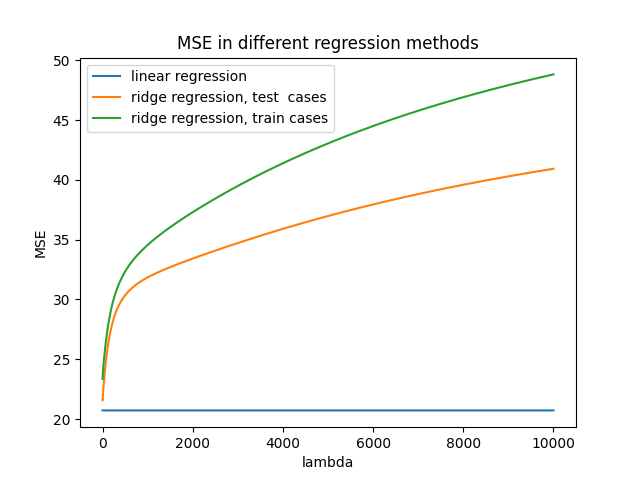
\includegraphics[]{Figure_1.png}\\
		 随着权重$\lambda$不断增大,测试集MSE和训练集MSE都在逐渐变大,但增速逐渐放缓。考虑应该是增加的正则化项影响到了模型对真实情况的模拟,正则化项占比越大,对真实情况的拟合程度越差,反映出人为的偏好。测试代码见附件。
	\end{solution}
\question [20] \textbf{线性判别分析}

教材3.4节介绍了“线性判别分析”模型LDA (Linear Discriminative Analysis), 本题首先针对LDA从分布假设的角度进行推导和分析.
考虑$N$分类问题, 训练集 $\left\{(\vx_1,y_1),(\vx_2,y_2),\ldots,(\vx_m,y_m)\right\}$, 其中, 第 $n$ 类样例从高斯分布 $\mathcal{N}(\vmu_n,\mSigma_n)$ 中独立同分布采样得到 (其中, $n=1,2,\cdots,N$). 记该类样例数量为 $m_n$. 类别先验为 $p\left(y=n\right)=\pi_n$, 反映了各类别出现的概率. 若$\vx\in \mathbb{R}^d \sim \mathcal{N}(\vmu,\mSigma)$, 则其概率密度函数为
\begin{align}
	p(\vx)=\frac{1}{(2\pi)^{\frac{d}{2}}\det\left(\mSigma\right)^\frac{1}{2}}\exp\left(-\frac{1}{2}(\vx-\vmu)^\top\mSigma^{-1}(\vx-\vmu)\right).
\end{align}
假设不同类别的条件概率为高斯分布, 当不同类别的协方差矩阵$\mSigma_n$相同时, 对于类别的预测转化为类别中心之间的线性问题, % 因此在这一假设下, 该方法也被称为线性判别分析 , 简称LDA. 
下面对这一模型进行进一步分析.
假设$\mSigma_n = \mSigma$, 分析LDA的分类方式以及参数估计步骤.
\begin{enumerate}
	\item \label{Q1q1}样例 $\vx$ 的后验概率$p\left(y=n\mid \vx\right)$表示了样例属于第$n$类的可能性, 当计算样例针对$N$个类别的后验概率后, 找出后验概率最大的类别对样例的标记进行预测, 即 $\arg\max_n$ $p\left(y=n\mid \vx\right)$. 等价于考察 $\ln p(y=n\mid \vx)$的大小,  请证明在此假设下, 
	\begin{equation}
	\arg\max_y p\left(y\mid \vx\right)=\arg\max_n\; \underbrace{\vx^{\top} \mSigma^{-1} \vmu_{n}-\frac{1}{2} \vmu_{n}^{\top} \mSigma^{-1} \vmu_{n}+\ln \pi_{n}}_{\delta_n(\vx)}    \;.
	\end{equation}
	其中 $\delta_{n}(\vx)$ 为LDA在分类时的判别函数. 
	\item \label{Q1q2} 在LDA模型中, 需要估计各类别的先验概率, 以及条件概率中高斯分布的参数. 针对二分类问题 ($N=2$), 使用如下方式估计类别先验、均值与协方差矩阵: 
	\begin{align}
	    \hat{\pi}_{n}&=\frac{m_n}{m}; \quad
	    \hat{\vmu}_{n}=\frac{1}{m_n}\sum_{y_{i}=n} \vx_{i}\;,\\
	    \hat{\mSigma}&=\frac{1}{m-N}\sum_{n=1}^{N} \sum_{y_{i}=n}\left(\vx_{i}-\hat{\vmu}_{n}\right)\left(\vx_{i}-\hat{\vmu}_{n}\right)^{\top}\;.
	\end{align}
	LDA使用这些经验量替代真实参数, 计算判别式 $\delta_n(\vx)$ 并按照第\ref{Q1q1}问中的准则做出预测. 请证明:
	\begin{equation}
	    \vx^{\top} \hat{\mSigma}^{-1}\left(\hat{\vmu}_{2}-\hat{\vmu}_{1}\right)>\frac{1}{2}\left(\hat{\vmu}_{2}+\hat{\vmu}_{1}\right)^{\top} \hat{\mSigma}^{-1}\left(\hat{\vmu}_{2}-\hat{\vmu}_{1}\right)-\ln \left(m_{2} / m_{1}\right)
	\end{equation}时 LDA 将样例预测为第 2 类. 请分析这一判别方式的几何意义.
	\item 在LDA中, 对样例$\vx$的判别可视为在投影的空间中和某个阈值进行比较. 上述推导通过最大后验概率的方法得到对投影后样例分布的需求, 而Fisher判别分析 (Fisher Discriminant Analysis, FDA)也是一种常见的线性判别分析方法, 直接对样例投影后数据的分布情况进行约束. 
FDA一般通过广义瑞利商进行求解, 请基于教材3.4节对“线性判别分析”的介绍,对广义瑞利商的性质进行分析, 探讨FDA多分类推广的性质.
下面请说明对于$N$类分类问题, FDA投影的维度最多为$N-1$, 即投影矩阵$\mW\in\mathbb{R}^{d\times (N-1)}$.\\
    提示:矩阵的秩具有如下性质:
    对于矩阵$\mathbf{A}\in\mathbb{R}^{m \times n}$, 矩阵$\mathbf{B}\in\mathbb{R}^{n \times r}$, 则
    \begin{equation}
        \operatorname{rank}(\mathbf{A})+\operatorname{rank}(\mathbf{B})-n \leq \operatorname{rank}(\mathbf{A B}) \leq \min \{\operatorname{rank}(\mathbf{A}), \operatorname{rank}(\mathbf{B})\}\;.
    \end{equation}
    对于任意矩阵$\mA$, 以下公式成立
    \begin{equation}
    \operatorname{rank}(\mA)=\operatorname{rank}\left(\mathbf{A}^{\top}\right)=\operatorname{rank}\left(\mathbf{A} \mathbf{A}^{\top}\right)=\operatorname{rank}\left(\mathbf{A}^{\top} \mathbf{A}\right)\;.
    \end{equation}
\end{enumerate}
	\begin{solution}
	    \\1.\\
		当各个类别的协方差矩阵相同时,若$x\in\mathbb R^d\sim \mathcal N(\mu_i,\Sigma)$,则$p(x)$可以转化为更简单的形式:
		$$p(x)=k\exp\left( -\frac12(x-\mu_i)^\top\Sigma^{-1}(x-\mu_i) \right)$$
		其中k为和类别无关的常数,设置为1不影响结论,由贝叶斯公式:
		$$p(y\mid \vx)=\frac{p(y)p(\vx\mid y)}{p(\vx)}$$
		可以得到:
		$$\begin{aligned}
			\arg\max_y p(y\mid\vx)
			&=\arg\max_n \frac{p(y=n)p(\vx\mid y=n)}{p(\vx)}\\
			&=\arg\max_n \frac{p(y=n)p(\vx_n)}{p(\vx)}\\
			&=\arg\max_n\ln\frac{p(y=n)p(\vx_n)}{p(\vx)}\\
			&=\arg\max_n\ln p(y=n)+\ln p (\vx_n)-\ln p(\vx)\\
		\end{aligned}$$
		因为$p(\vx)$不随$n$的改变而变化,由此原式转化为:
		$$\begin{aligned}
			\arg\max_y p(y\mid\vx)
			&=\arg\max_n\ \ln p(y=n)+\ln p (\vx_n)\\
			&=\arg\max_n\ \ln\pi_n-\frac12(x-\mu_n)^\top\Sigma^{-1}(x-\mu_n)\\
			&=\arg\max_n\ \ln\pi_n+ \vx^\top\Sigma^{-1}\mu_n-\frac12\vx^\top\Sigma^{-1}\vx-\frac12\mu_n^\top\Sigma^{-1}{\mu_n}\\
		\end{aligned}
		$$
		 加入不随$n$变化的项$\frac12\vx^\top\Sigma^{-1}\vx$不改变原优化问题,因此有:
		 $$\arg\max_y p(y\mid\vx)=\arg\max_n\ \ln\pi_n+ \vx^\top\Sigma^{-1}\mu_n-\frac12\mu_n^\top\Sigma^{-1}{\mu_n}$$
		\\2.
			由判别函数
			$$ \delta_n(x)=x^\top\hat\Sigma^{-1}\hat\mu_n-\frac12\hat\mu_n^\top\hat\Sigma^{-1}\hat\mu_n+\ln \hat\pi_n$$
			可以写出预测为1类和2类的表达式:
			$$\delta_1(x)=x^\top\hat\Sigma^{-1}\hat\mu_1-\frac12\hat\mu_1^\top\hat\Sigma^{-1}\hat\mu_1+\ln ({m_1}/m)$$
			$$\delta_2(x)=x^\top\hat\Sigma^{-1}\hat\mu_2-\frac12\hat\mu_2^\top\hat\Sigma^{-1}\hat\mu_2+\ln ({m_2}/m)$$
			在预测中,预测的$\delta_n(x)$值越大,最终预测为这个分类的概率就越大,因此我们有:
			$$\delta_2(x)>\delta_1(x)$$
			$$\begin{aligned}
				&\iff \delta_2(x)-\delta(_1x)>0\\
				&\iff x^\top\hat\Sigma^{-1}(\hat\mu_2-\hat\mu_1)-(\frac12\hat\mu_2^\top\hat\Sigma^{-1}\hat\mu_2-\frac12\hat\mu_1^\top\hat\Sigma^{-1}\hat\mu_1)+\ln (m_2/m_1)>0\\
				&\iff x^\top\hat\Sigma^{-1}(\hat\mu_2-\hat\mu_1)>\frac12(\hat\mu_2^\top\hat\Sigma^{-1}\hat\mu_2-\hat\mu_1^\top\hat\Sigma^{-1}\hat\mu_1)-\ln (m_2/m_1)\\
			\end{aligned}$$
			$\therefore$为证明原来预测正确,只需要证明:
			$$\frac12(\hat\mu_2^\top\hat\Sigma^{-1}\hat\mu_2-\hat\mu_1^\top\hat\Sigma^{-1}\hat\mu_1)\le\frac12(\hat\mu_2+\hat\mu_1)^\top\hat\Sigma^{-1}(\hat\mu_2-\hat\mu_1)$$
		即证明$$\hat\mu_1^\top\Sigma^{-1}\hat\mu_2\ge \hat\mu_2^\top\Sigma^{-1}\hat\mu_1\quad\quad\quad\quad\quad\quad\quad\ (a)$$
		因为左表达式为一个数,$ \hat\mu_1^\top\Sigma^{-1}\hat\mu_2\in \mathbb R$\\\\
		$\therefore$我们有:$ \hat\mu_1^\top\Sigma^{-1}\hat\mu_2 = (\hat\mu_1^\top\Sigma^{-1}\hat\mu_2)^\top=\hat\mu_2^\top\Sigma^{-1}\hat\mu_1$\\\\
		$\therefore$(a)式成立,因此原预测值成立\\
		预测方法$\arg\max_n\delta_n(x)$的几何意义为在向量空间中,使其在n号分布上的出现频率最大时的取值n,也就是反映其分布在此处的疏密程度,将样例判别为在此分布最密集的。
		\\3.\\.
		原问题的求解等价于求解广义特征值问题:$$S_bW=\lambda S_wW$$
		其闭式解为$S_w^{-1}S_b$的$d'$个最大非零广义特征值所对应的特征向量组成的矩阵,记这个矩阵为$\mathfrak W$\\
		$$\because S_b=\sum\limits^N_{i=1}m_i(\mu_i-\mu)(\mu_i-\mu)^\top$$
		且$rank((\mu_i-\mu)(\mu_i-\mu)^\top)= rank((\mu_i-\mu))=1$ \\
		$\therefore S_b$为N个秩为1的矩阵之和,即$$rank(S_b)\le N$$
		又$\mu_i-\mu$并非线性无关,因此其和之秩小于N,有\\
		$$rank(S_b)<N\iff rank(S_b)\le N-1$$
		又$$rank(S_w^{-1}S_b)\le \min(rank(S_w^{-1}),rank(S_b))\le rank(S_b)\le N-1 $$
		$\therefore S_w^{-1}S_b$一共有不超过N-1个特征值,因此有$$rank(\mathfrak W)\le N-1$$
	\end{solution}


\question [20] \textbf{多分类学习}

	教材3.5节介绍了“多分类学习”的多种方式, 本题针对OvO和OvR两种多分类学习方法进行分析:
\begin{enumerate}
    \item 分析两种多分类方法的优劣. 思考这两种多分类推广方式是否存在难以处理的情况?
    \item 在OvR的每一个二分类子任务中, 目标类别作为正类, 而其余所有类别作为负类. 此时, 是否需要显式考虑正负类别的不平衡带来的影响?
\end{enumerate}
	\begin{solution}
		1.\\
	    OvR只需要训练$N$个分类器,而OvO需要$N(N-1)/2$个分类器,因此OvO一般比OVR需要更大的存储开销和测试时间开销。然而在训练分类器时,OvR的所有分类器都需要使用所有的训练用例,而OvO的每个分类器只需要用到涉及到的两个用例的训练样本,因此在类别很多时,训练时的时间开销OvO要小于OvR\\
		2.\\
		不需要显式考虑。我们对每个类都进行了相同的处理,其产生的类别不平衡效果会相互抵消,通常不会对分类器的性能造成影响。
	\end{solution}

\end{questions}


\end{document}